\phantomsection
\section{Code Development}
Below are the various APIs developed from the class diagrams and models of D2.
\subsection{Treatment, Hospital, and Department Management}

\begin{figure}[H]
    \centering
    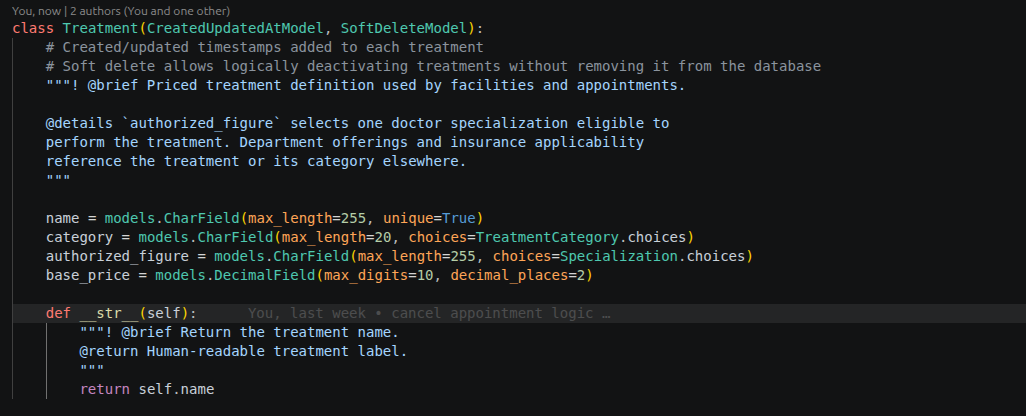
\includegraphics[width=\textwidth]{ScreenshotD3/code_snippets/treatmentModel.png}
    \caption{Treatment model definition declaring the necessary attributes.}
    \label{fig:treatment_model}
\end{figure}

\begin{figure}[H]
    \centering
    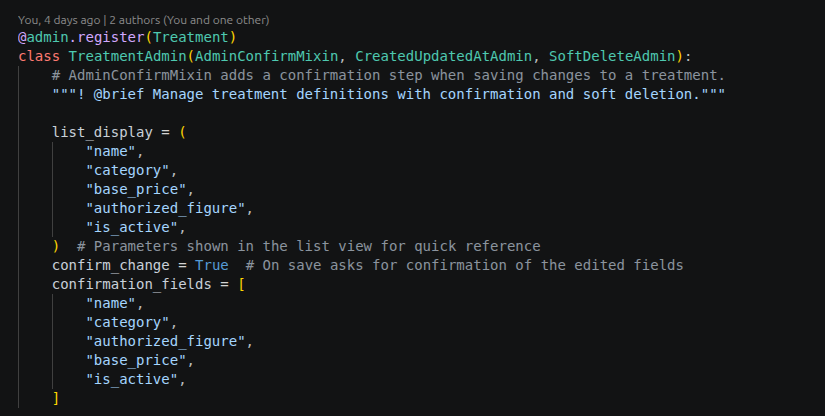
\includegraphics[width=\textwidth]{ScreenshotD3/code_snippets/treatmentAdmin.png}
    \caption{Treatment admin configuration utilizing mixins for soft deletion and edit confirmation.}
    \label{fig:treatment_admin}
\end{figure}

The functionality allowing an administrator to manage treatments, hospitals, and departments follows a consistent pattern across the application:

\begin{itemize}
    \item The model defines the relevant class attributes.
    \item The Django admin automatically generates the interface for entity creation. Non-default behaviors---such as soft deletion and edit confirmation prompts---are implemented using custom admin classes and mixins.
\end{itemize}

The management functionalities for Hospitals and Departments are implemented using the exact same approach; the primary difference lies solely in the specific attributes declared within their respective models.

\vspace{0.5cm}
\noindent\textbf{Linked Use Cases:}
\begin{itemize}
    \item \textbf{UC1} - Create Treatment / Hospital / Department
    \item \textbf{UC5} - Edit Treatment / Hospital / Department
    \item \textbf{UC8} - Deactivate or close Treatment / Hospital / Department
\end{itemize}

\phantomsection
\subsection{Insurance Policy Administration Management}

\begin{figure}[H]
    \centering
    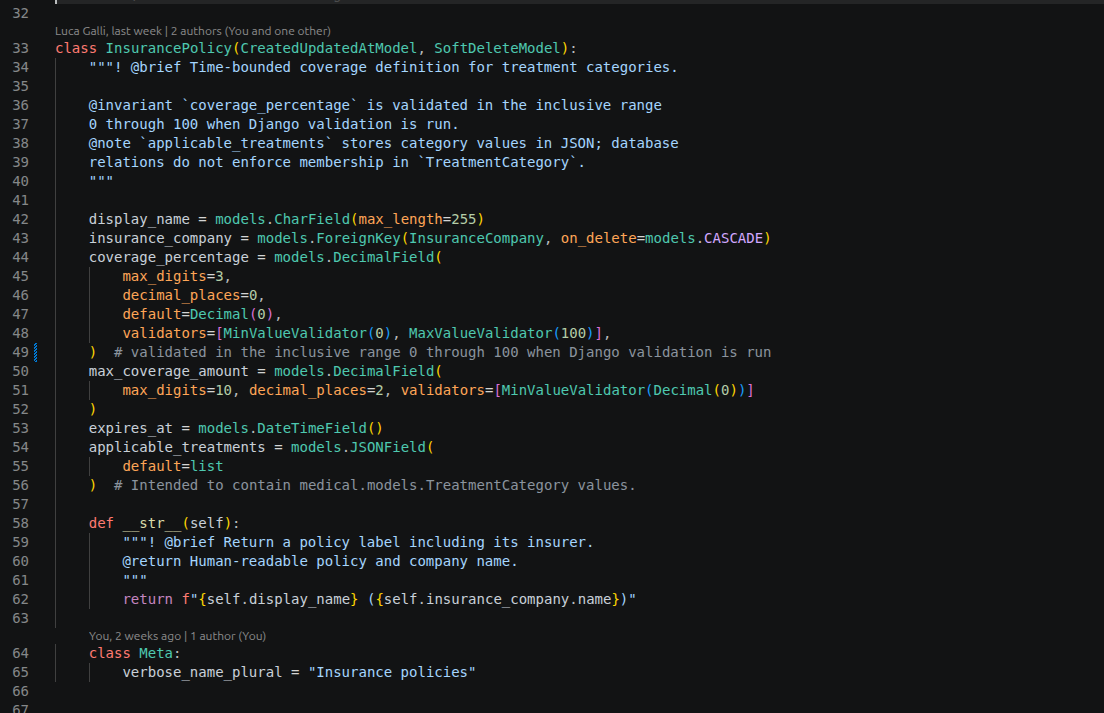
\includegraphics[width=\textwidth]{ScreenshotD3/code_snippets/policyModel.png}
    \caption{Insurance Policy model definition declaring the necessary attributes and validators.}
    \label{fig:policy_model}
\end{figure}

\begin{figure}[H]
    \centering
    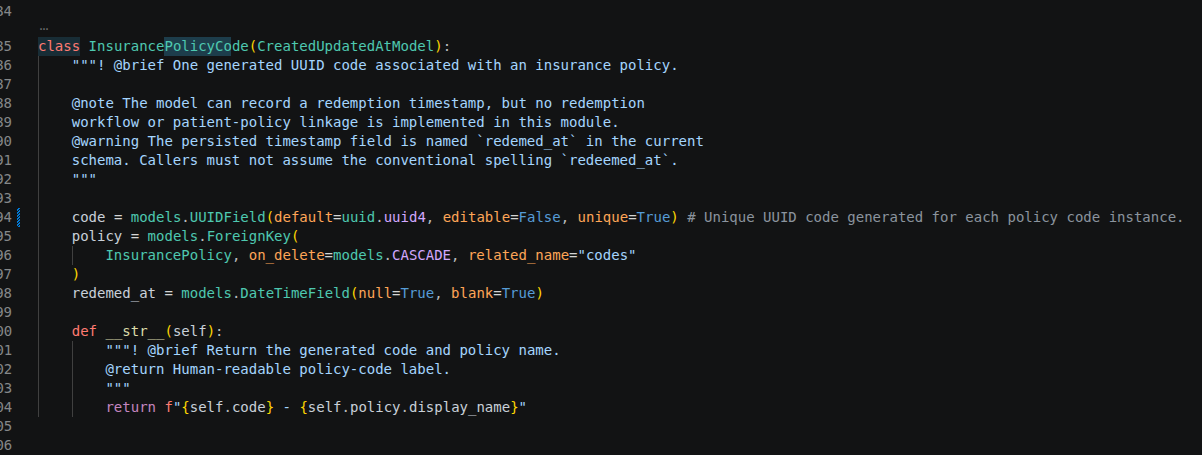
\includegraphics[width=\textwidth]{ScreenshotD3/code_snippets/policyCodeModel.png}
    \caption{Insurance Policy Code model definition.}
    \label{fig:policy_code_model}
\end{figure}

\begin{figure}[H]
    \centering
    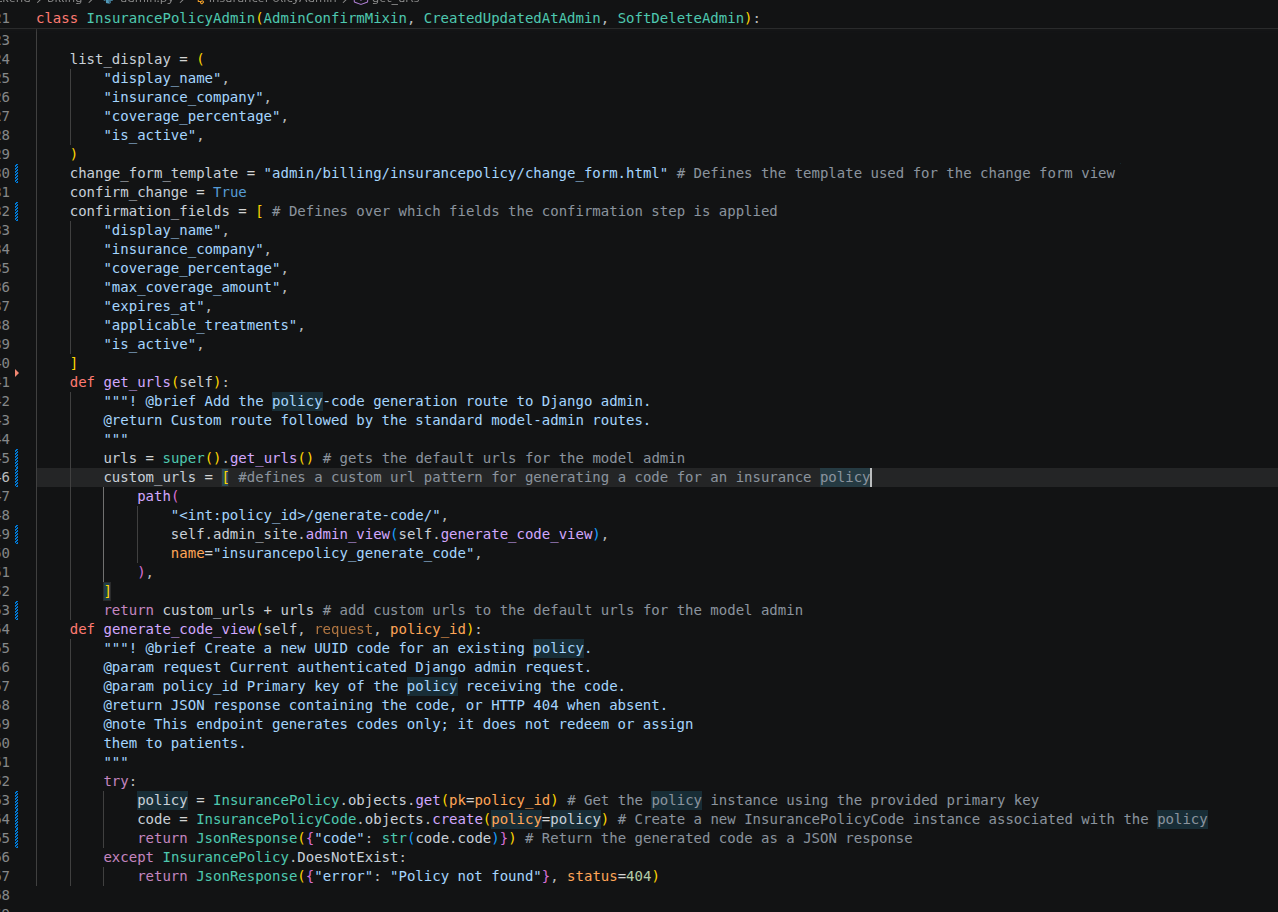
\includegraphics[width=\textwidth]{ScreenshotD3/code_snippets/policyAdmin.png}
    \caption{Insurance Policy admin configuration utilizing mixins and custom endpoints.}
    \label{fig:policy_admin}
\end{figure}

It is worth noting that specific field-level validations have been integrated directly into the models to strictly enforce the business rules outlined in the use cases. For instance, the \texttt{coverage\_percentage} is constrained within an inclusive range of 0 to 100.

Furthermore, the administration interface for insurance policies is notably more complex than standard entities to accommodate the dynamic generation of policy codes. This complexity is managed through several key customizations:

\begin{itemize}
    \item \textbf{Custom UI Integration:} The admin class defines a \texttt{change\_form\_template} to utilize a custom HTML layout. This allows the injection of specific UI elements directly within the standard Django edit form.
    \item \textbf{Custom Routing:} The \texttt{get\_urls()} method is overridden to append a new, protected API endpoint (\texttt{<int:policy\_id>/generate-code/}) to the standard model-admin URL patterns.
    \item \textbf{Dedicated View Logic:} The \texttt{generate\_code\_view()} method acts as the controller for this new route. It securely fetches the requested policy instance, generates a unique, one-off \texttt{InsurancePolicyCode} (UUID), and returns it to the client as a JSON response.
\end{itemize}

\vspace{0.5cm}
\noindent\textbf{Linked Use Cases:}
\begin{itemize}
    \item \textbf{UC2} - Create Insurance Policy
    \item \textbf{UC6} - Update Insurance Policy
    \item \textbf{UC9} - Deactivate Insurance Policy
    \item \textbf{UC22} - Generate Insurance Policy Code
\end{itemize}

\phantomsection
\subsection{Doctor Creates Prescription / Exemption / Examination}

\begin{figure}[H]
    \centering
    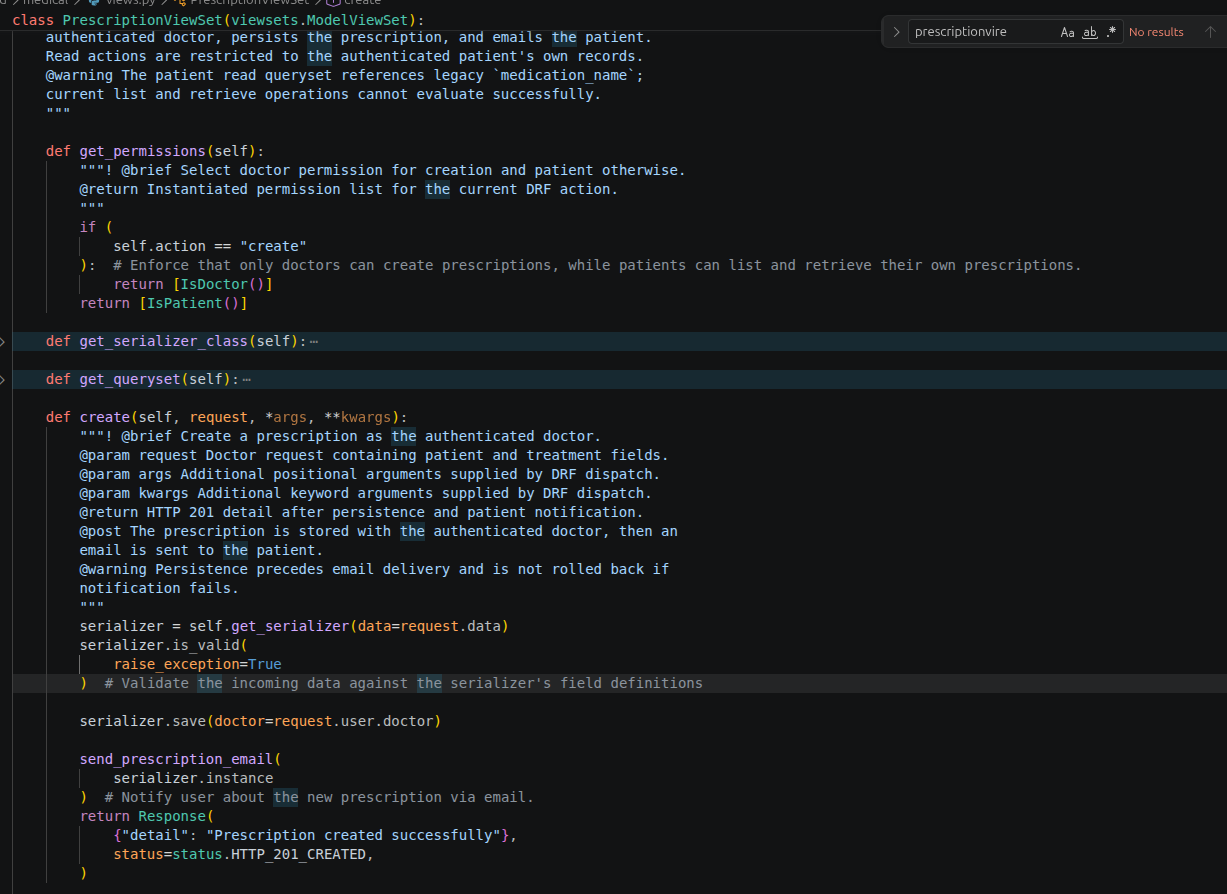
\includegraphics[width=\textwidth]{ScreenshotD3/code_snippets/prescriptionCreateView.png}
    \caption{Prescription creation view implementation.}
    \label{fig:prescription_create_view}
\end{figure}

\begin{figure}[H]
    \centering
    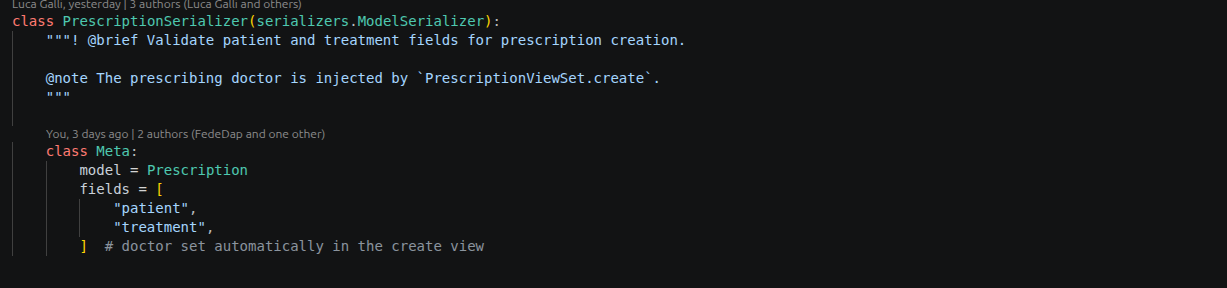
\includegraphics[width=\textwidth]{ScreenshotD3/code_snippets/prescriptionCreateSerializer.png}
    \caption{Prescription creation serializer implementation.}
    \label{fig:prescription_create_serializer}
\end{figure}

\begin{figure}[H]
    \centering
    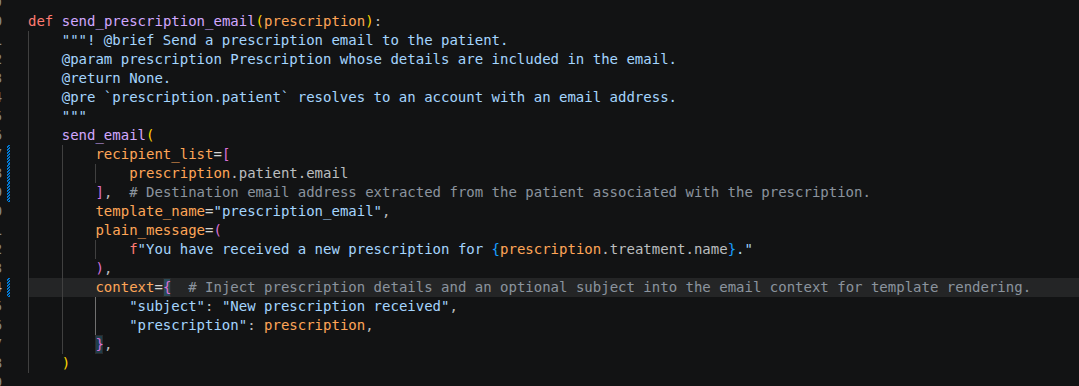
\includegraphics[width=\textwidth]{ScreenshotD3/code_snippets/prescriptionEmail.png}
    \caption{Prescription email notification implementation.}
    \label{fig:prescription_email}
\end{figure}

The creation of a prescription is handled by a dedicated DRF \texttt{ViewSet} that overrides both the permission logic and the \texttt{create()} method to enforce the business rules associated with this use case.

\begin{itemize}
    \item \textbf{Permission Enforcement:} The \texttt{get\_permissions()} method dynamically selects the applicable permission class based on the requested action. Only authenticated doctors are allowed to perform the \texttt{create} action, while patients retain read-only access (list and retrieve) restricted to their own prescriptions.
    \item \textbf{Serializer Validation:} The \texttt{PrescriptionSerializer} exposes only the \texttt{patient} and \texttt{treatment} fields to the client. The prescribing doctor is deliberately excluded from the writable fields, as it is automatically injected server-side from the authenticated user.
    \item \textbf{Creation Logic:} The overridden \texttt{create()} method validates the incoming payload, persists the prescription by associating it with the doctor profile of the authenticated user (\texttt{request.user.doctor}), and finally triggers an email notification to the patient.
    \item \textbf{Email Notification:} The \texttt{send\_prescription\_email()} function retrieves the patient's email address from the prescription instance and dispatches a templated email informing them of the new prescription, including the treatment name in the message body and context.
\end{itemize}

\vspace{0.2cm}

\vspace{0.2cm}
\noindent The management of Exemptions and examinations follows the exact same approach described above; the \texttt{ViewSet}, serializer, and email notification logic mirror the structure shown for Prescriptions, with the only difference being the specific model and fields involved.

\vspace{0.5cm}
\noindent\textbf{Linked Use Cases:}
\begin{itemize}
    \item \textbf{UC3} - Create Prescription / Exemption
    \item \textbf{UC4} - Upload Examination
\end{itemize}


\phantomsection
\subsection{Account Management}

\begin{figure}[H]
    \centering
    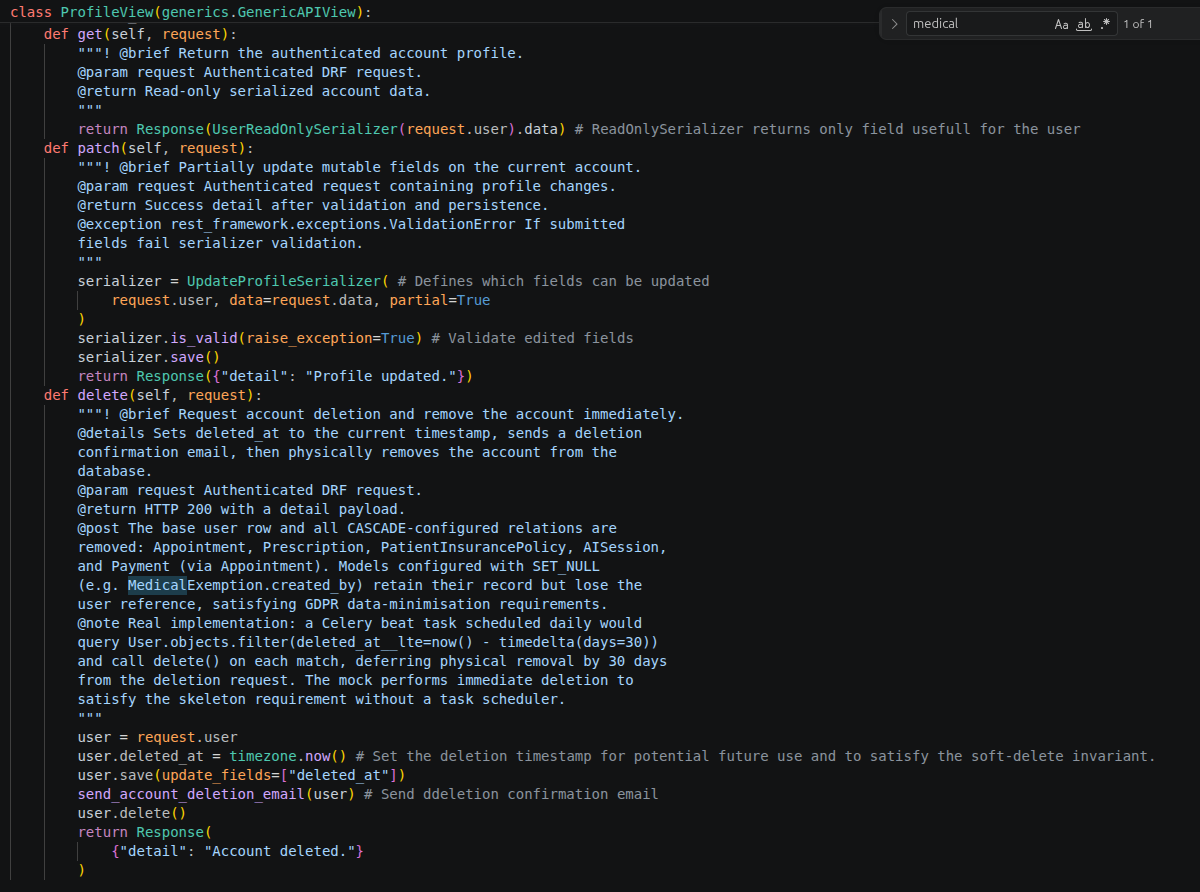
\includegraphics[width=\textwidth]{ScreenshotD3/code_snippets/profileActions.png}
    \caption{Profile actions implementation.}
    \label{fig:profile_actions}
\end{figure}

\begin{figure}[H]
    \centering
    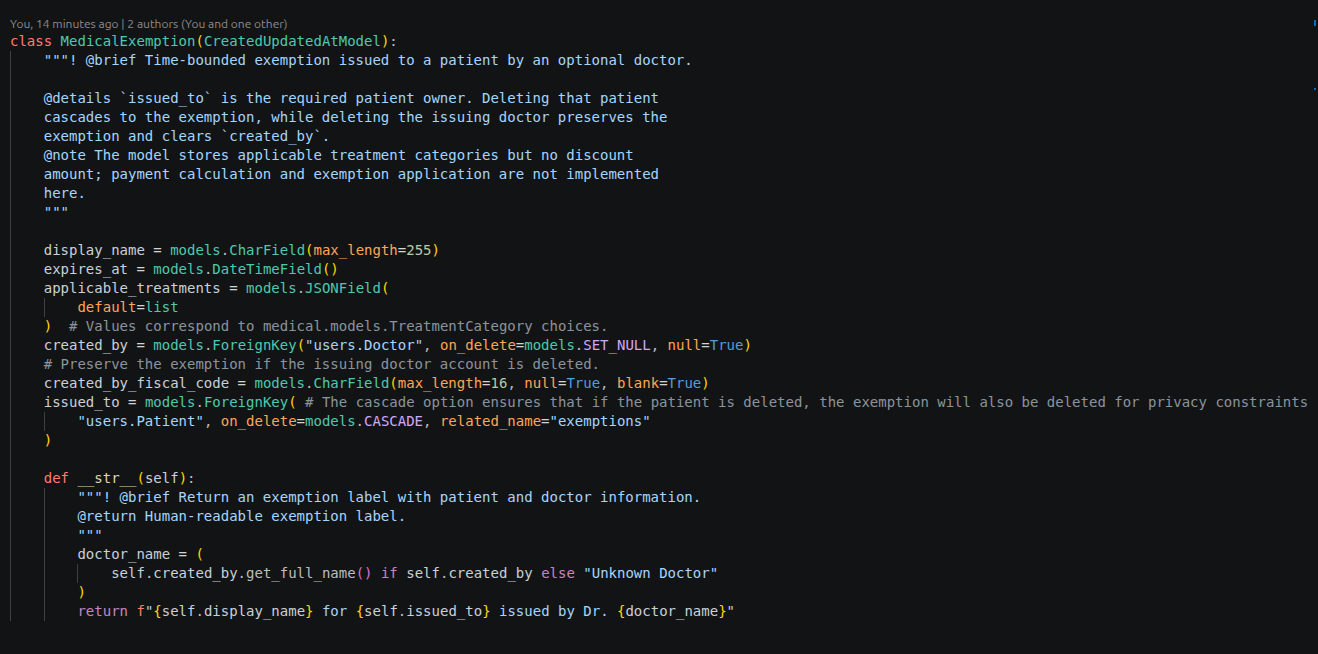
\includegraphics[width=\textwidth]{ScreenshotD3/code_snippets/exemptionModel.png}
    \caption{Medical Exemption model definition showing the \texttt{CASCADE} and \texttt{SET\_NULL} relations used for cascading deletion.}
    \label{fig:medical_exemption_model}
\end{figure}

To satisfy \textbf{NFR0 - Security and Privacy} and to enforce GDPR compliance, account deletion has been designed to support a \textit{soft delete} mechanism.

\begin{itemize}
\item \textbf{Soft Delete Flag:} The data model already includes a \texttt{deleted\_at} timestamp field, intended to mark an account as pending deletion without immediately destroying the underlying data. In the current implementation, however, the \texttt{delete()} handler of \texttt{ProfileView} sets this timestamp and then immediately proceeds with the physical deletion of the account (\texttt{user.delete()}), after sending a confirmation email to the user via \texttt{send\_account\_deletion\_email()}. The flag is therefore already in place to support the grace-period mechanism described below, even though it is not yet leveraged to defer the actual deletion.    \item \textbf{Future Periodic Cleanup:} In the intended production implementation, a periodic Celery beat task would run daily, querying for all users whose \texttt{deleted\_at} timestamp is older than 30 days (\texttt{User.objects.filter(deleted\_at\_\_lte=now() - timedelta(days=30))}) and physically deleting them. 
    \item \textbf{Mock Behavior:} Since no task scheduler is included in this skeleton, the current implementation performs the physical deletion (\texttt{user.delete()}) immediately after setting \texttt{deleted\_at}, in order to demonstrate the cascading behavior described below without requiring Celery infrastructure.
\end{itemize}

\vspace{0.2cm}
\noindent\textbf{Cascading Data Removal.} The physical deletion of the user record triggers a cascade of deletions across all related entities, as configured at the model level via \texttt{on\_delete} relations. As shown in Figure~\ref{fig:medical_exemption_model} for the \texttt{MedicalExemption} model, two distinct strategies are applied depending on the nature of the relationship:

\begin{itemize}
    \item \textbf{CASCADE:} Models that represent data intrinsically owned by the deleted account are configured with \texttt{on\_delete=models.CASCADE}. When the patient account is removed, all of these related records are deleted along with it, ensuring no personal data is left behind.
    \item \textbf{SET\_NULL:} Conversely, models that may need to be preserved for medical or administrative continuity are configured with \texttt{on\_delete=models.SET\_NULL}. If the issuing doctor's account is deleted, the exemption record itself is retained, but the foreign key reference is cleared, satisfying the GDPR data-minimisation principle while preserving the exemption for the patient.
\end{itemize}

\vspace{0.5cm}
\noindent\textbf{Linked Use Cases:}
\begin{itemize}
    \item \textbf{UC7} - Update User profile
    \item \textbf{UC41} - Account Deletion
\end{itemize}



\phantomsection
\subsection{Registration and Validation}

\begin{figure}[H]
    \centering
    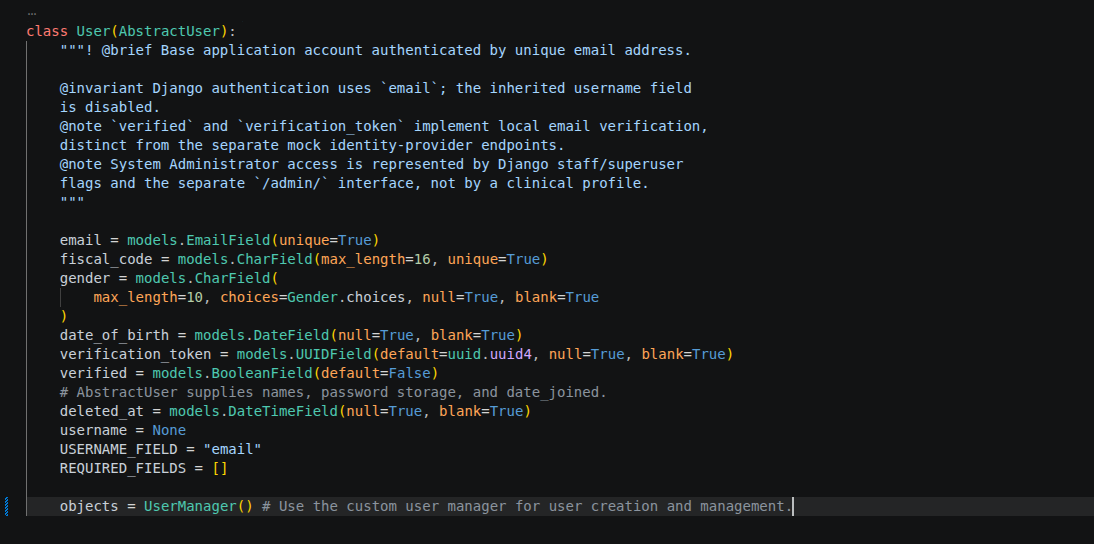
\includegraphics[width=\textwidth]{ScreenshotD3/code_snippets/userClass.png}
    \caption{User class definition showing the attributes and methods for user management.}
    \label{fig:user_class}
\end{figure}
\begin{figure}[H]
    \centering
    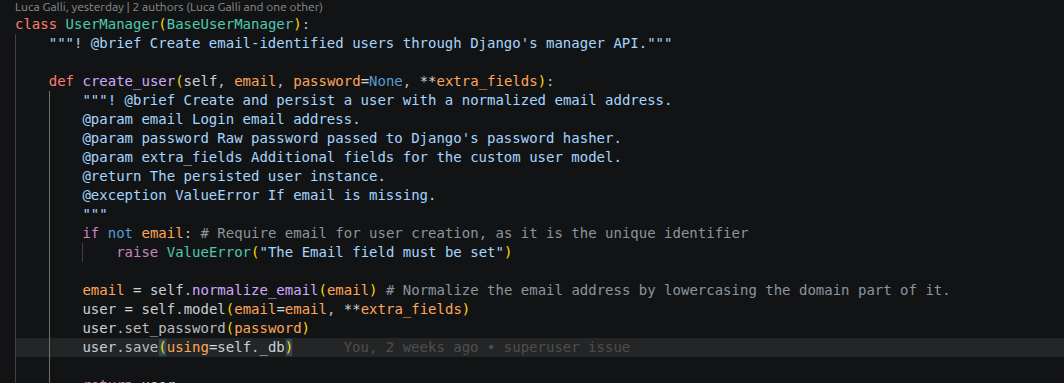
\includegraphics[width=\textwidth]{ScreenshotD3/code_snippets/userManager.png}
    \caption{User manager implementation showing the custom user creation logic.}
    \label{fig:user_manager}
\end{figure}
\begin{figure}[H]
    \centering
    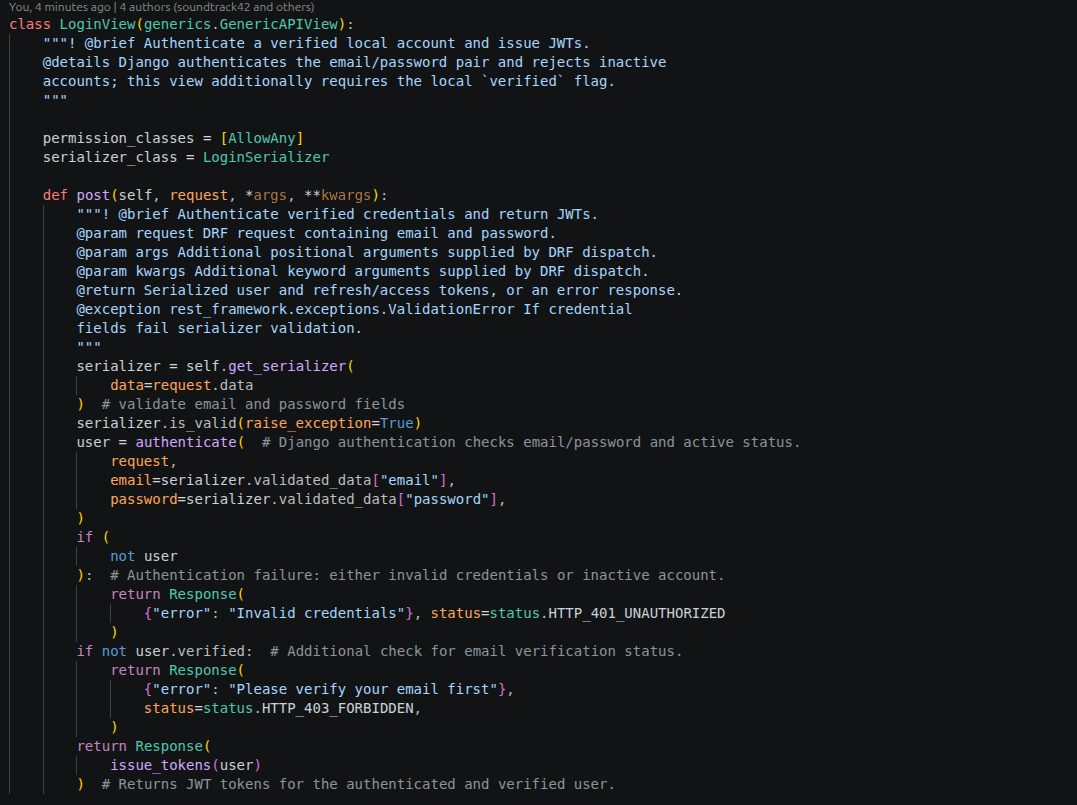
\includegraphics[width=\textwidth]{ScreenshotD3/code_snippets/loginView.png}
    \caption{Login view implementation showing the user authentication logic.}
    \label{fig:login_view}
\end{figure}
\begin{figure}[H]
    \centering
    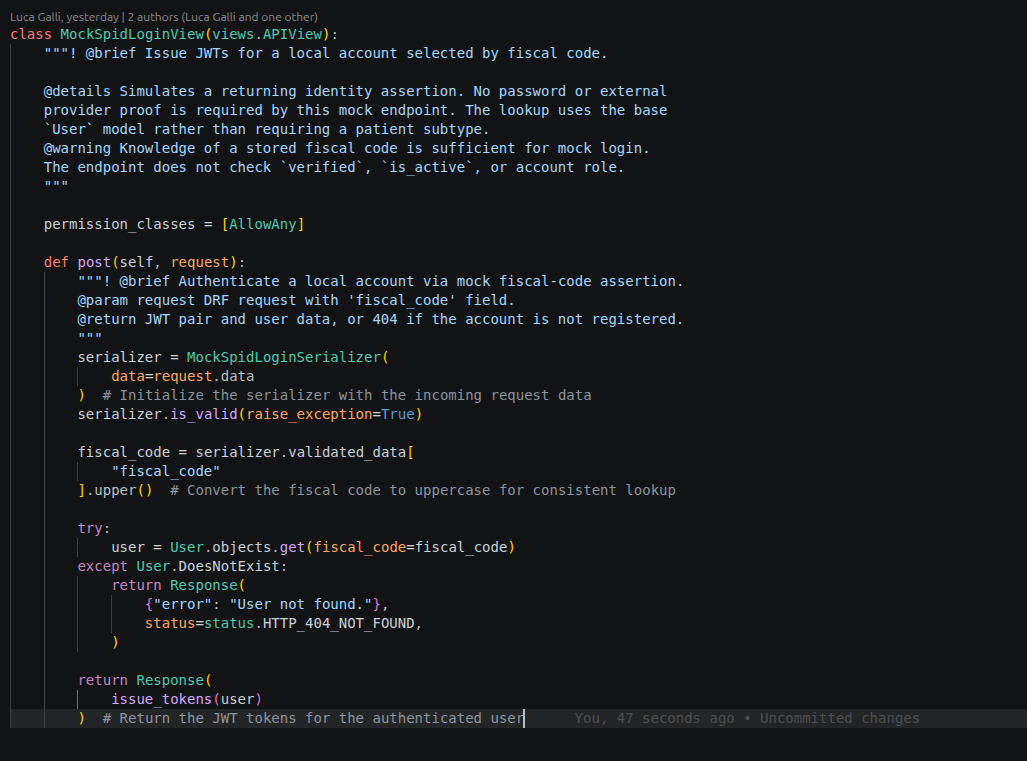
\includegraphics[width=\textwidth]{ScreenshotD3/code_snippets/mockLogin.png}
    \caption{Mock SPID login implementation.}
    \label{fig:mock_login}
\end{figure}
\begin{figure}[H]
    \centering
    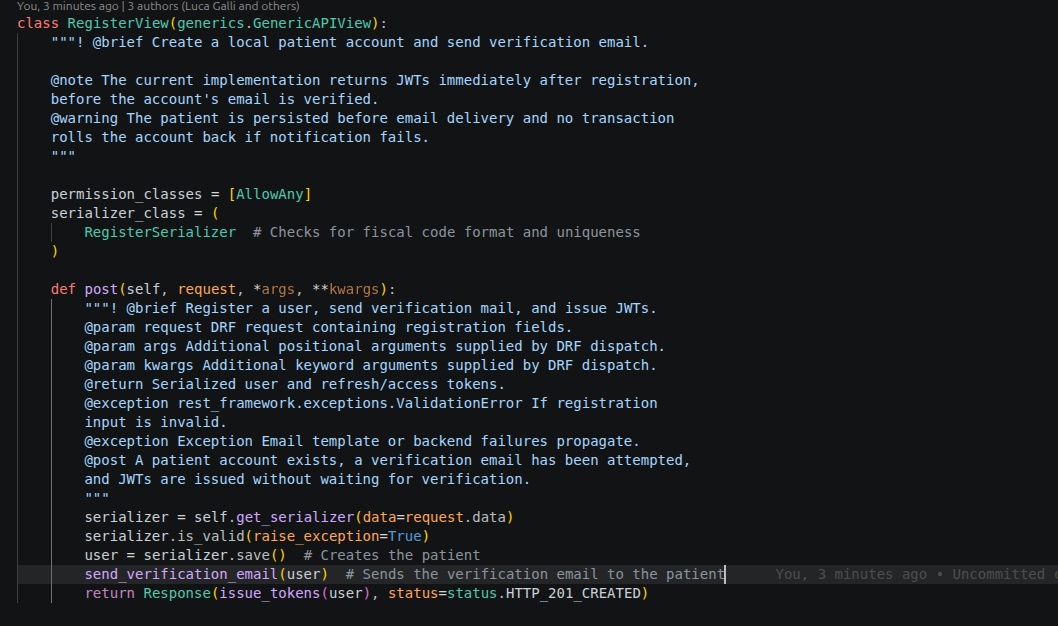
\includegraphics[width=\textwidth]{ScreenshotD3/code_snippets/registerView.png}
    \caption{Registration view implementation showing the user registration logic.}
    \label{fig:register_view}
\end{figure}
\begin{figure}[H]
    \centering
    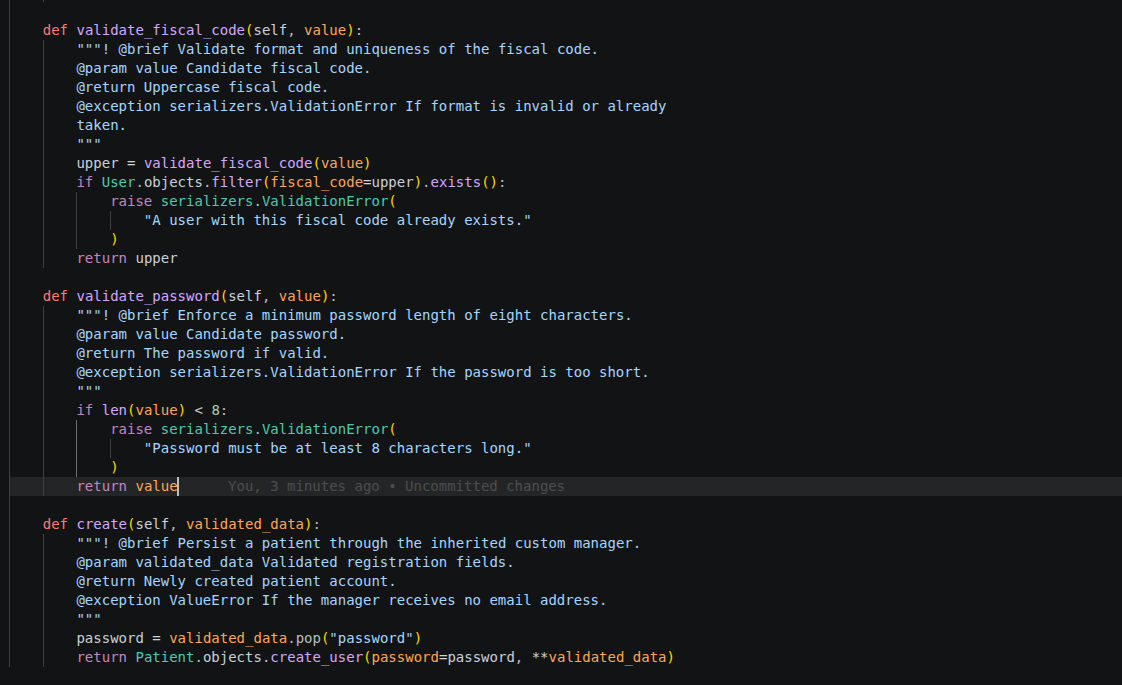
\includegraphics[width=\textwidth]{ScreenshotD3/code_snippets/registerSerializer.png}
    \caption{Registration serializer implementation showing the validation logic.}
    \label{fig:register_serializer}
\end{figure}
\begin{figure}[H]
    \centering
    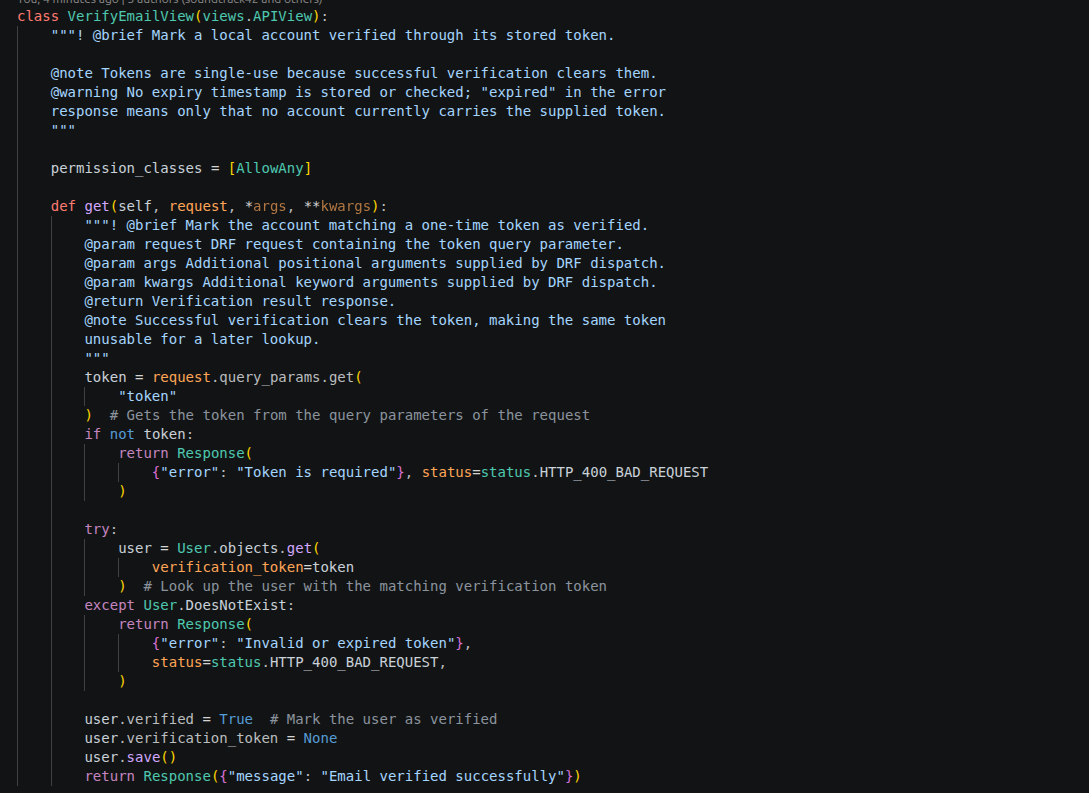
\includegraphics[width=\textwidth]{ScreenshotD3/code_snippets/verifyEmail.png}
    \caption{Email verification implementation showing the verification logic.}
    \label{fig:verify_email}
\end{figure}
\begin{figure}[H]
    \centering
    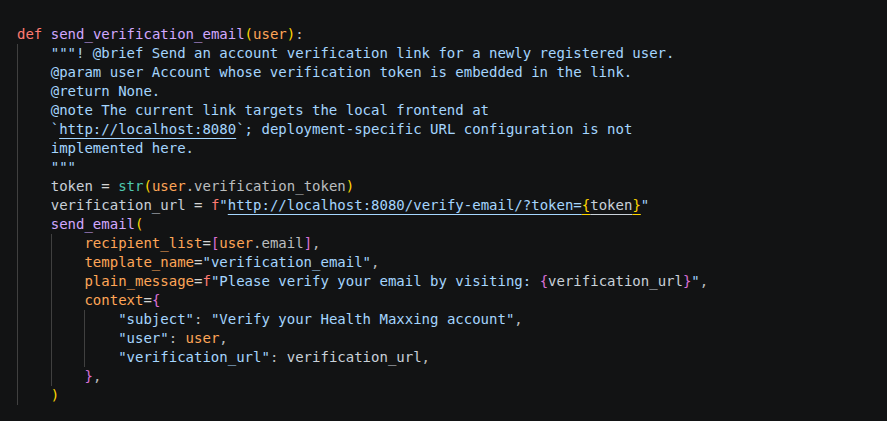
\includegraphics[width=\textwidth]{ScreenshotD3/code_snippets/sendVerificationEmail.png}
    \caption{Email verification implementation showing the verification logic.}
    \label{fig:send_verification_email}
\end{figure}

The \texttt{User} model extends Django's \texttt{AbstractUser} and is configured to authenticate via \texttt{email} instead of a username, which is explicitly disabled by setting \texttt{USERNAME\_FIELD = "email"} and \texttt{username = None}. In addition to the fields inherited from \texttt{AbstractUser} (such as name and password storage), the model defines application-specific attributes: a unique \texttt{fiscal\_code}, an optional \texttt{gender} and \texttt{date\_of\_birth}, and the pair \texttt{verified} / \texttt{verification\_token}, which together implement local email verification independently from the mock identity-provider endpoints. User creation is delegated to a custom \texttt{UserManager}, which normalizes the email address, enforces its presence, and hashes the password before persisting the account.

\vspace{0.2cm}
\noindent\textbf{Registration.} The \texttt{RegisterView} exposes an open (\texttt{AllowAny}) endpoint that validates the incoming payload through \texttt{RegisterSerializer} --- which checks the format and uniqueness of the fiscal code --- and persists the new patient account. Immediately after creation, \texttt{send\_verification\_email()} is called to deliver a verification link containing the account's \texttt{verification\_token}.

\vspace{0.2cm}
\noindent\textbf{Email Verification.} The \texttt{send\_verification\_email()} function builds a one-time verification URL embedding the user's \texttt{verification\_token} and dispatches it via the templated email system. The corresponding \texttt{VerifyEmailView} exposes a public endpoint that looks up the account matching the token supplied as a query parameter; if found, the account is marked as \texttt{verified} and its token is cleared, making it single-use. If no account matches the supplied token, a generic ``invalid or expired token'' error is returned.

\vspace{0.2cm}
\noindent\textbf{Login.} The \texttt{LoginView} validates the submitted email and password through \texttt{LoginSerializer} and then relies on Django's \texttt{authenticate()} to verify the credentials and the account's active status. On top of this, the view performs an additional check on the local \texttt{verified} flag: if the credentials are valid but the account has not yet completed email verification, an HTTP 403 response is returned instructing the user to verify their email first. Only after passing both checks are JWT tokens issued to the client via \texttt{issue\_tokens()}.

\vspace{0.5cm}
\noindent\textbf{Linked Use Cases:}
\begin{itemize}
    \item \textbf{UC23} - User Registration and Validation
    \item \textbf{UC24} - User Login
\end{itemize}

\phantomsection
\subsection{Medical Record access}

\begin{figure}[H]
    \centering
    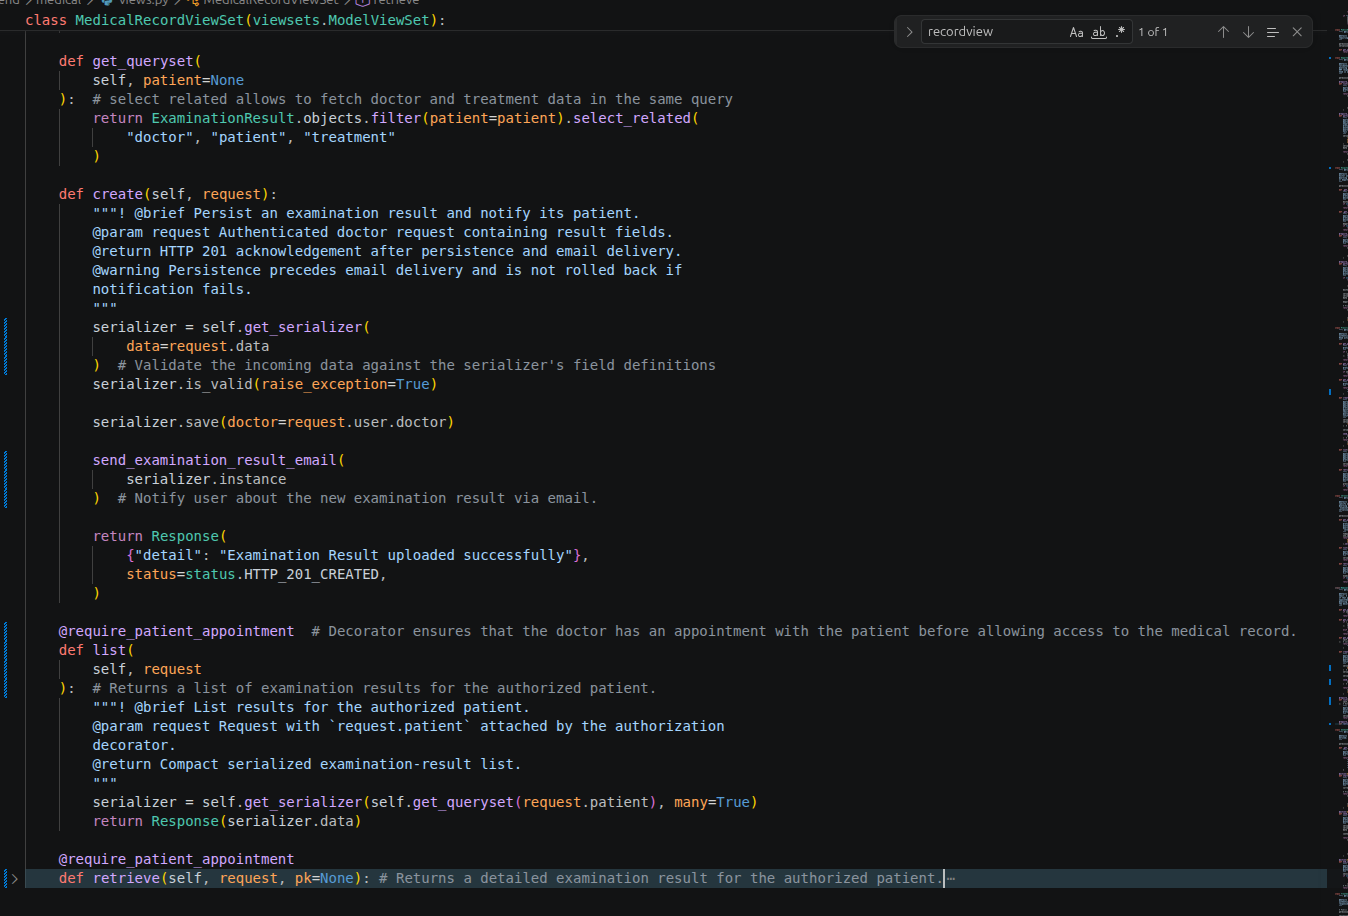
\includegraphics[width=\textwidth]{ScreenshotD3/code_snippets/recordView.png}
    \caption{Medical record access implementation showing the record view.}
    \label{fig:record_view}
\end{figure}
\begin{figure}[H]
    \centering
    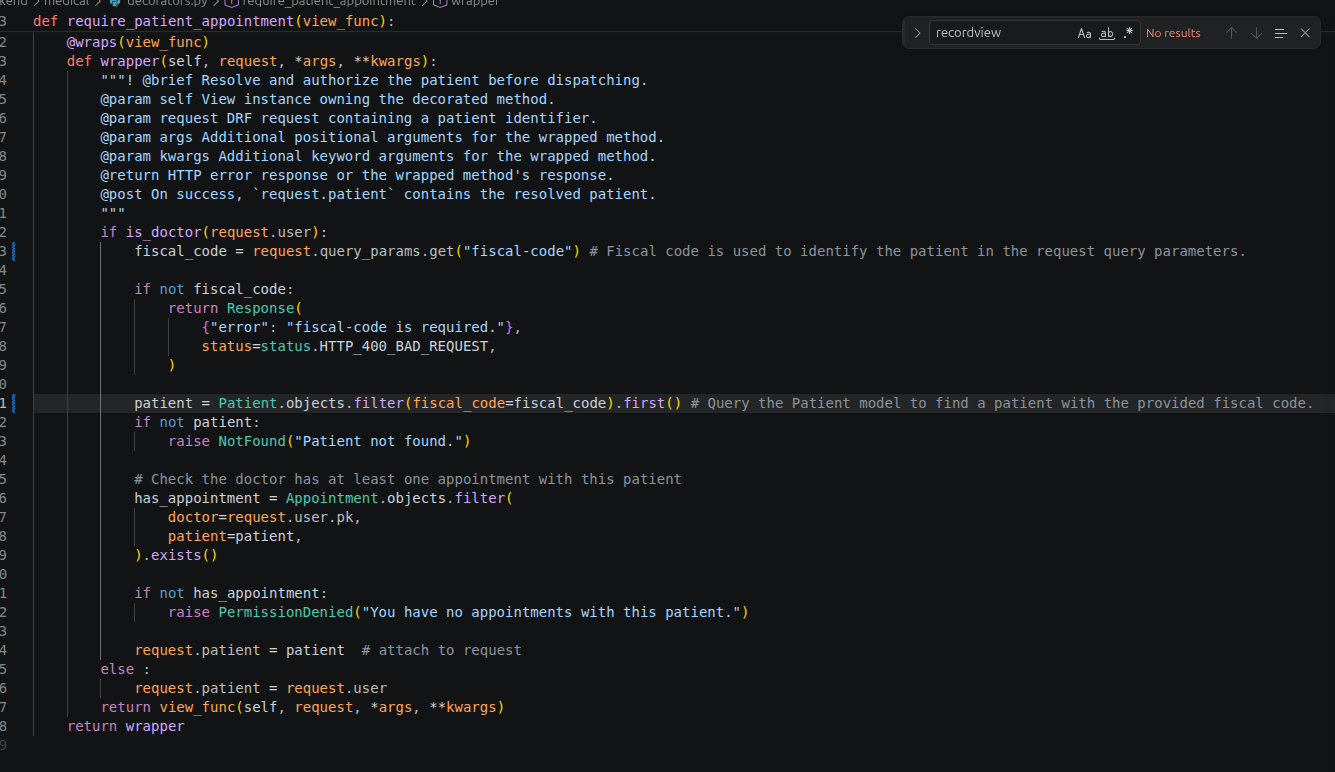
\includegraphics[width=\textwidth]{ScreenshotD3/code_snippets/requireAppointmentWrap.png}
    \caption{Appointment requirement implementation.}
    \label{fig:require_appointment_wrap}
\end{figure}

Access to medical records (examination results) is handled by \texttt{MedicalRecordViewSet}, which differentiates behavior based on both the requested action and the role of the authenticated user.

\begin{itemize}
    \item \textbf{Permission Enforcement:} The \texttt{get\_permissions()} method restricts the \texttt{create} action to doctors only (\texttt{IsDoctor}), while all other actions simply require an authenticated user (\texttt{IsAuthenticated}), since both patients and doctors are allowed to read records, subject to the additional authorization described below.
    \item \textbf{Serializer Selection:} The \texttt{get\_serializer\_class()} method returns a different serializer depending on the action: a fully validated \texttt{ExaminationResultSerializer} is used for creation, a lightweight \texttt{ExaminationResultListSerializer} is used for listing, and a more detailed \texttt{ExaminationResultDetailSerializer} is used for retrieving a single record.
    \item \textbf{Creation Logic:} The \texttt{create()} method validates the incoming payload, persists the examination result associating it with the authenticated doctor (\texttt{request.user.doctor}), and notifies the patient by calling \texttt{send\_examination\_result\_email()}. As with other notification flows in the system, persistence precedes email delivery and is not rolled back if the notification fails.
    \item \textbf{Queryset Construction:} The \texttt{get\_queryset()} method filters \texttt{ExaminationResult} objects by the resolved patient and uses \texttt{select\_related()} on \texttt{doctor}, \texttt{patient}, and \texttt{treatment} to avoid additional queries when serializing related data.
\end{itemize}

\vspace{0.2cm}
\noindent\textbf{Authorization via \texttt{require\_patient\_appointment}.} The \texttt{list()} and \texttt{retrieve()} actions are wrapped by the \texttt{require\_patient\_appointment} decorator, which is responsible for resolving \emph{whose} medical records the request is allowed to access and attaching the result to \texttt{request.patient}:

\begin{itemize}
    \item \textbf{Patient Requests:} If the authenticated user is not a doctor, they are assumed to be a patient, and \texttt{request.patient} is simply set to \texttt{request.user}, granting access to their own records.
    \item \textbf{Doctor Requests:} If the authenticated user is a doctor, the request must include a \texttt{fiscal-code} query parameter identifying the target patient. The decorator looks up the corresponding \texttt{Patient} record (raising \texttt{NotFound} if it does not exist) and then verifies that the doctor has at least one \texttt{Appointment} with that patient, raising \texttt{PermissionDenied} otherwise.
\end{itemize}

\vspace{0.2cm}

\vspace{0.5cm}
\noindent\textbf{Linked Use Cases:}
\begin{itemize}
    \item \textbf{UC40} - Medical Record Access (patient)
    \item \textbf{UC42} - Medical record access (doctor)
\end{itemize}